\documentclass{warpdoc}
\newlength\lengthfigure                  % declare a figure width unit
\setlength\lengthfigure{0.158\textwidth} % make the figure width unit scale with the textwidth
\usepackage{psfrag}         % use it to substitute a string in a eps figure
\usepackage{subfigure}
\usepackage{rotating}
\usepackage{pstricks}
\usepackage[innercaption]{sidecap} % the cute space-saving side captions
\usepackage{scalefnt}
\usepackage{bm}
\usepackage{amsmath}
\usepackage{graphicx}
\usepackage{rotating}
\usepackage{bm}
\usepackage{caption}
\usepackage{float}

%%%%%%%%%%%%%=--NEW COMMANDS BEGINS--=%%%%%%%%%%%%%%%%%%%%%%%%%%%%%%%%%%
\newcommand{\alb}{\vspace{0.2cm}\\} % array line break
\newcommand{\ordi}{{\rm d}}
%\let\vec\bf
\renewcommand{\vec}[1]{\bm{#1}}
\newcommand{\mfa}{\scriptscriptstyle}
\newcommand{\mfb}{\scriptstyle}
\newcommand{\mfc}{\textstyle}
\newcommand{\mfd}{\displaystyle}
\newcommand{\hlinex}{\vspace{-0.34cm}~~\\ \hline \vspace{-0.31cm}~~\\}
\newcommand{\hlinextop}{\vspace{-0.46cm}~~\\ \hline \hline \vspace{-0.32cm}~~\\}
\newcommand{\hlinexbot}{\vspace{-0.37cm}~~\\ \hline \hline \vspace{-0.50cm}~~\\}
\newcommand{\tablespacing}{\vspace{-0.4cm}}
\renewcommand{\fontsizetable}{\footnotesize\scalefont{0.9}}
\setcounter{tocdepth}{3}
\let\citen\cite

%%%%%%%%%%%%%=--NEW COMMANDS ENDS--=%%%%%%%%%%%%%%%%%%%%%%%%%%%%%%%%%%%%
%%%%%%%%%%%%%=--NEW COMMANDS BEGINS--=%%%%%%%%%%%%%%%%%%%%%%%%%%%%%%%%%%


\author{
  Bernard Parent
}

\email{
  bparent@arizona.edu
}

\department{
  Aerospace and Mechanical Engineering
}

\institution{
  University of Arizona
}

\title{Nine Species NH3 Plasma Kinetics 
}

\date{
  July 2023
}

%\setlength\nomenclaturelabelwidth{0.13\hsize}  % optional, default is 0.03\hsize
%\setlength\nomenclaturecolumnsep{0.09\hsize}  % optional, default is 0.06\hsize

\nomenclature{

  \begin{nomenclaturelist}{Roman symbols}
   \item[$a$] speed of sound
  \end{nomenclaturelist}
}


\abstract{
abstract
}

\begin{document}
  \pagestyle{headings}
  \pagenumbering{arabic}
  \setcounter{page}{1}
%%  \maketitle
  \makewarpdoctitle
%  \makeabstract
%  \tableofcontents
%  \makenomenclature
%  \listoftables
%%  \listoffigures












%
\begin{table}
  \center\fontsizetable
  \begin{threeparttable}
    \tablecaption{Bavafa (2008) 9-species 8-reactions NH$_3$ plasma chemical model.\tnote{a}}
    \label{tab:Bavafa}
    \fontsizetable
    \begin{tabular*}{\textwidth}{l@{\extracolsep{\fill}}lll}
    \toprule
    No.&Reaction\tnote{(b)} & Rate Coefficient  & Refs. \\
    \midrule
    1  & $\rm e^- + NH_2   \rightarrow NH_3^+ + e^- + e^-$  
       &  ${\rm min}({\rm exp}(1.2346\cdot 10^{-14} \cdot {\rm ln}^9 E^\star +  0.3115 \cdot {\rm ln} E^\star), 1.5640 \cdot 10^{-07})$~cm$^3$/s
       & \cite{psst:2005:hagelaar}, \cite{jap:1996:yousfi} \\
    2 & $\rm e^- + NH_3 \rightarrow NH_2^+ + H + e^- + e^-$  
       &  ${\rm min}({\rm exp}(0.4853 \cdot {\rm ln} E^\star +  5.5515 \cdot 10^{-131} \cdot {\rm ln}^{79} E^\star), 2.4490 \cdot 10^{-10})$~cm$^3$/s
       & \cite{psst:2005:hagelaar}, \cite{book:2013:mark}\\
    3  & $\rm e^- + NH_3 \rightarrow NH_2 + H + e^-$   
       & \multicolumn{1}{p{8cm}}{${\rm min}({\rm exp}(2.0636\cdot 10^{-07} {\rm ln}^5 E^\star -  4.3548 \cdot 10^{-11} \cdot {\rm ln}^{07} E^\star), 1.04 \cdot 10^{-08} \cdot {\rm exp}(-1.129 \cdot 10^{19} \cdot E^\star) + 2.046 \cdot 10^{-09} \cdot {\rm exp}(-3.627 \cdot 10^{05} \cdot E^\star))$ cm$^3$/s}
       & \cite{psst:2005:hagelaar}, \cite{jap:1996:yousfi}\\
    4  & $\rm e^- + NH_3 \rightarrow NH + H + H + e^-$   
       & ${\rm min}({\rm exp}(1.4602\cdot 10^{-07} \cdot {\rm ln}^5 E^\star -  1.3747 \cdot 10^{-21} \cdot {\rm ln}^{13} E^\star), 1.200 \cdot 10^{-08})$~cm$^3$/s 
       & \cite{psst:2005:hagelaar}, \cite{jap:1996:yousfi}\\
    5  & $\rm NH_2 + H \rightarrow NH_3 $   
       & $10^{-13}$ cm$^3$/s 
       & \cite{book:1987:krivonosova}, \cite{psst:1995:dollet}\\
    6  & $\rm NH_2 + NH_2 \rightarrow NH + NH_3 $   
       & $ 1.4 \cdot 10^{-12}$ cm$^3$/s 
       & \cite{book:1987:krivonosova}, \cite{psst:1995:dollet}\\  
    7  & $\rm NH_3 + NH_3^+ \rightarrow NH_2 + NH_4^+ $   
       & $ 2.2 \cdot 10^{-09}$ cm$^3$/s 
       & \cite{book:1987:krivonosova}, \cite{psst:1995:dollet}\\  
    8  & $\rm NH_3 + NH_2^+ \rightarrow NH_2 + NH_3^+ $   
       & $ 10^{-09}$ cm$^3$/s 
       & \cite{psst:1995:dollet}\\       
    \bottomrule
    \end{tabular*}
\begin{tablenotes}
\item[{a}] Notation and units: $E^\star$ is the reduced effective electric field in the electron reference frame ($E^\star\equiv|\vec{E}+\vec{V}^{\rm e}\times \vec{B}|/N$) in units of V$\cdot$m$^2$; $N_A$ is Avogadro's number and it is approximately $6.022 \cdot 10^{23}$
\end{tablenotes}
   \end{threeparttable}
\end{table}
%


%
\begin{table}
  \center\fontsizetable
  \begin{threeparttable}
    \tablecaption{Omprakas (2023) 9-species 13-reactions NH$_3$ plasma chemical model.\tnote{a}}
    \label{tab:Bavafa}
    \fontsizetable
    \begin{tabular*}{\textwidth}{l@{\extracolsep{\fill}}lll}
    \toprule
    No.&Reaction\tnote{(b)} & Rate Coefficient  & Refs. \\
    \midrule
    1  & $\rm e^- + NH_2   \rightarrow NH_3^+ + e^- + e^-$  
       &  ${\rm min}({\rm exp}(1.2346\cdot 10^{-14} \cdot {\rm ln}^9 E^\star +  0.3115 \cdot {\rm ln} E^\star), 1.5640 \cdot 10^{-07})$~cm$^3$/s
       & \cite{psst:2005:hagelaar}, \cite{jap:1996:yousfi} \\
    2 & $\rm e^- + NH_3 \rightarrow NH_2^+ + H + e^- + e^-$  
       &  ${\rm min}({\rm exp}(0.4853 \cdot {\rm ln} E^\star +  5.5515 \cdot 10^{-131} \cdot {\rm ln}^{79} E^\star), 2.4490 \cdot 10^{-10})$~cm$^3$/s
       & \cite{psst:2005:hagelaar}, \cite{book:2013:mark}\\
    3  & $\rm e^- + NH_3 \rightarrow NH_2 + H + e^-$   
       & \multicolumn{1}{p{8cm}}{${\rm min}({\rm exp}(2.0636\cdot 10^{-07} {\rm ln}^5 E^\star -  4.3548 \cdot 10^{-11} \cdot {\rm ln}^{07} E^\star), 1.04 \cdot 10^{-08} \cdot {\rm exp}(-1.129 \cdot 10^{19} \cdot E^\star) + 2.046 \cdot 10^{-09} \cdot {\rm exp}(-3.627 \cdot 10^{05} \cdot E^\star))$ cm$^3$/s}
       & \cite{psst:2005:hagelaar}, \cite{jap:1996:yousfi}\\
    4  & $\rm e^- + NH_3 \rightarrow NH + H + H + e^-$   
       & ${\rm min}({\rm exp}(1.4602\cdot 10^{-07} \cdot {\rm ln}^5 E^\star -  1.3747 \cdot 10^{-21} \cdot {\rm ln}^{13} E^\star), 1.200 \cdot 10^{-08})$~cm$^3$/s 
       & \cite{psst:2005:hagelaar}, \cite{jap:1996:yousfi}\\
    5  & $\rm NH_2 + H \rightarrow NH_3 $   
       & $10^{-13}$ cm$^3$/s 
       & \cite{book:1987:krivonosova}, \cite{psst:1995:dollet}\\
    6  & $\rm NH_2 + NH_2 \rightarrow NH + NH_3 $   
       & $ 1.4 \cdot 10^{-12}$ cm$^3$/s 
       & \cite{book:1987:krivonosova}, \cite{psst:1995:dollet}\\  
    7  & $\rm NH_3 + NH_3^+ \rightarrow NH_2 + NH_4^+ $   
       & $ 2.2 \cdot 10^{-09}$ cm$^3$/s 
       & \cite{book:1987:krivonosova}, \cite{psst:1995:dollet}\\  
    8  & $\rm NH_3 + NH_2^+ \rightarrow NH_2 + NH_3^+ $   
       & $ 10^{-09}$ cm$^3$/s 
       & \cite{psst:1995:dollet}\\      
    9  & $\rm e^- + NH_3^+   \rightarrow NH + H + H$   
       & $ 1 \times 10^{-07} \cdot T_e^{-0.5}$ cm$^3$/s 
       & \cite{pop:2012:li}\\
    10  & $\rm e^- + NH_4^+   \rightarrow NH_3 + H$   
       & $ 3.0 \times 10^{18} \cdot N_A^{-1} \cdot T_e^{-0.67}$ cm$^3$/s 
       & \cite{jpc:2015:truscott}\\
    11  & $\rm e^- + NH_4^+   \rightarrow NH_2 + H + H$   
       & $ 3.0 \times 10^{18} \cdot N_A^{-1} \cdot T_e^{-0.67}$ cm$^3$/s 
       & \cite{jpc:2015:truscott}\\
    12  & $\rm e^- + NH_2^+   \rightarrow NH + H$   
       & $ 1 \times 10^{-07} \cdot T_e^{-0.5}$ cm$^3$/s 
       & \cite{jpap:2007:arakoni}\\
    13  & $\rm e^- + NH_3^+   \rightarrow H + NH_2$   
       & $ 1 \times 10^{-07} \cdot T_e^{-0.5}$ cm$^3$/s 
       & \cite{jpap:2007:arakoni}\\
    \bottomrule
    \end{tabular*}
\begin{tablenotes}
\item[{a}] Notation and units: $E^\star$ is the reduced effective electric field in the electron reference frame ($E^\star\equiv|\vec{E}+\vec{V}^{\rm e}\times \vec{B}|/N$) in units of V$\cdot$m$^2$; $N_A$ is Avogadro's number and it is approximately $6.022 \cdot 10^{23}$
\end{tablenotes}
   \end{threeparttable}
\end{table}
%
%
The reaction rate for reaction 1 to 4 is obtained using BOLSIG+. The cross-section for reaction no 1,3, and 4 is obtained from \cite{jap:1996:yousfi}, and the cross-section for reaction no 2 is obtained from \cite{book:2013:mark}. Comprision between the reaction rate obtained from BOLSIG+ and curve-fit is shown in the figure below.
%
%
\begin{figure}[H]
\centering     %%% not \center
\subfigure[]{\label{fig:a}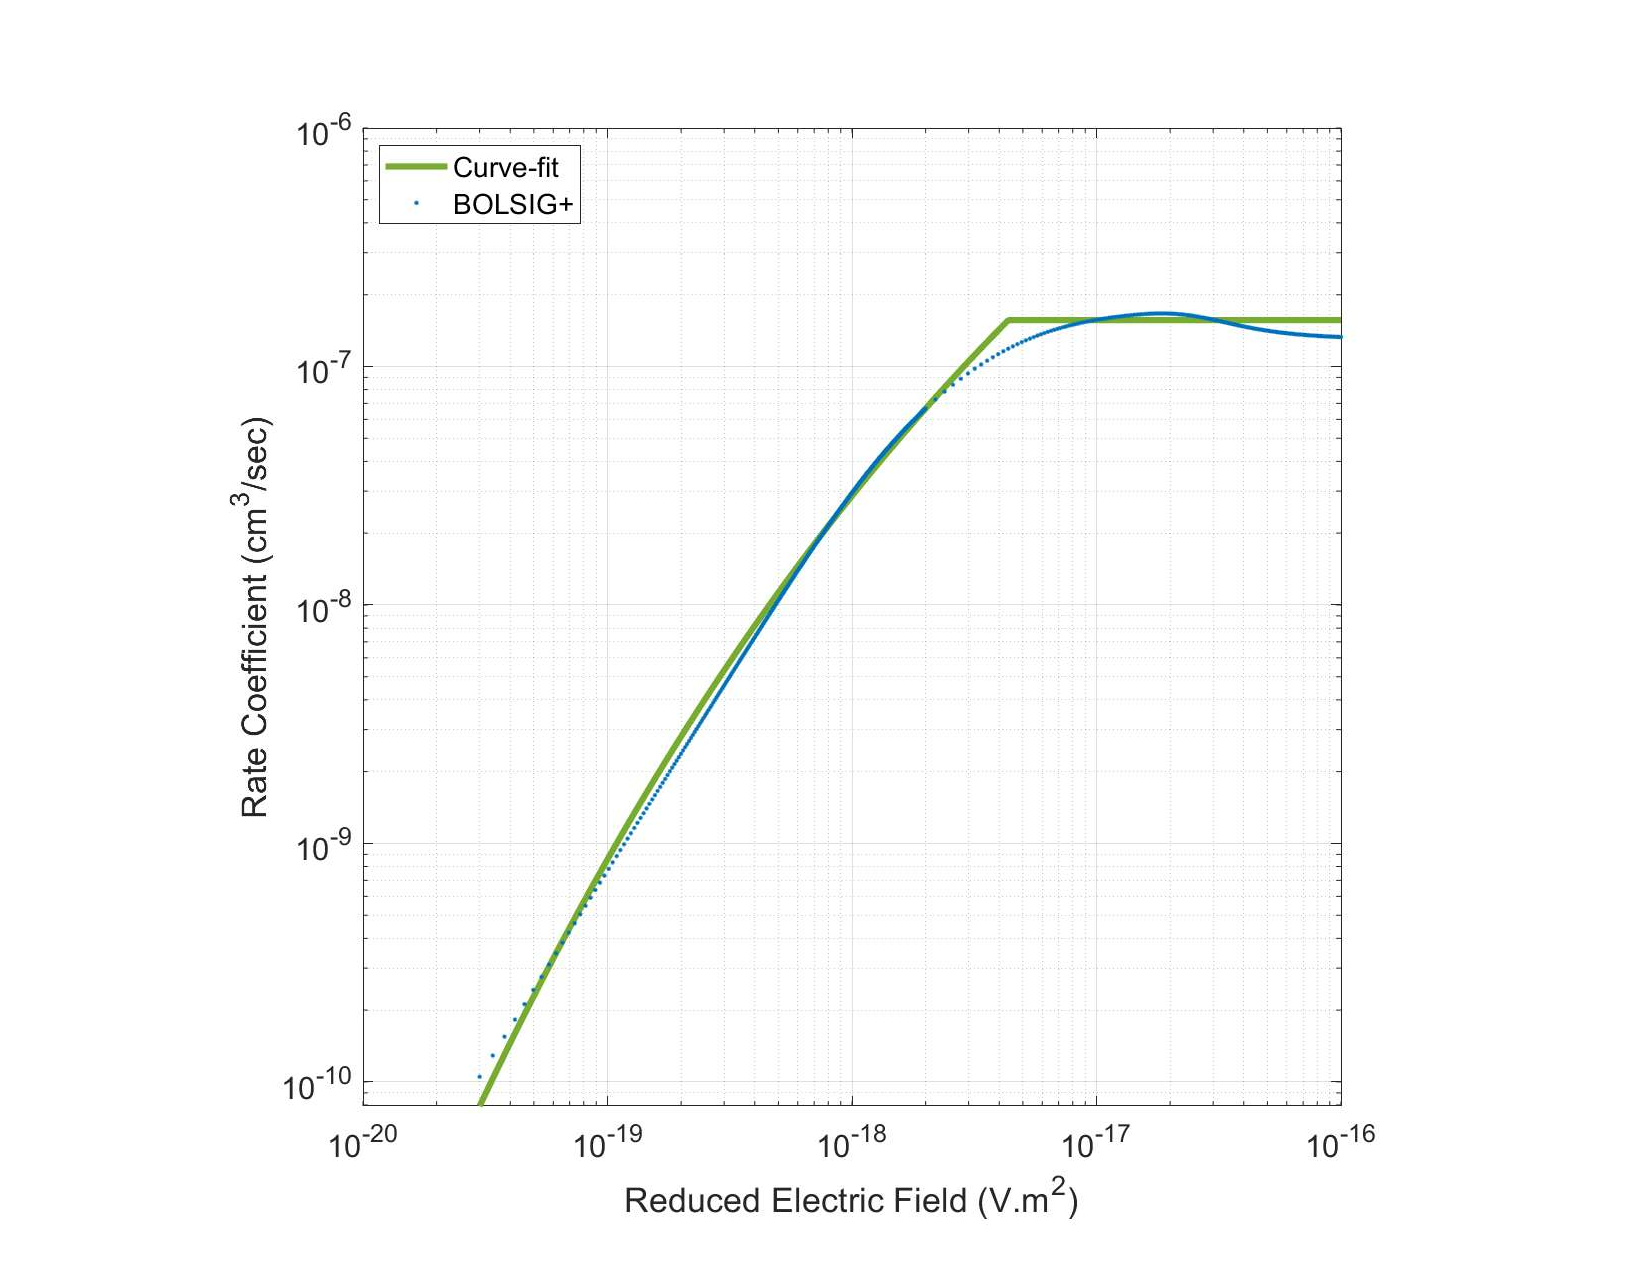
\includegraphics[clip, trim=0.5cm 0.5cm 0.5cm 0.5cm,width=0.95\linewidth]{Reaction_1_1.pdf}}
\subfigure[]{\label{fig:b}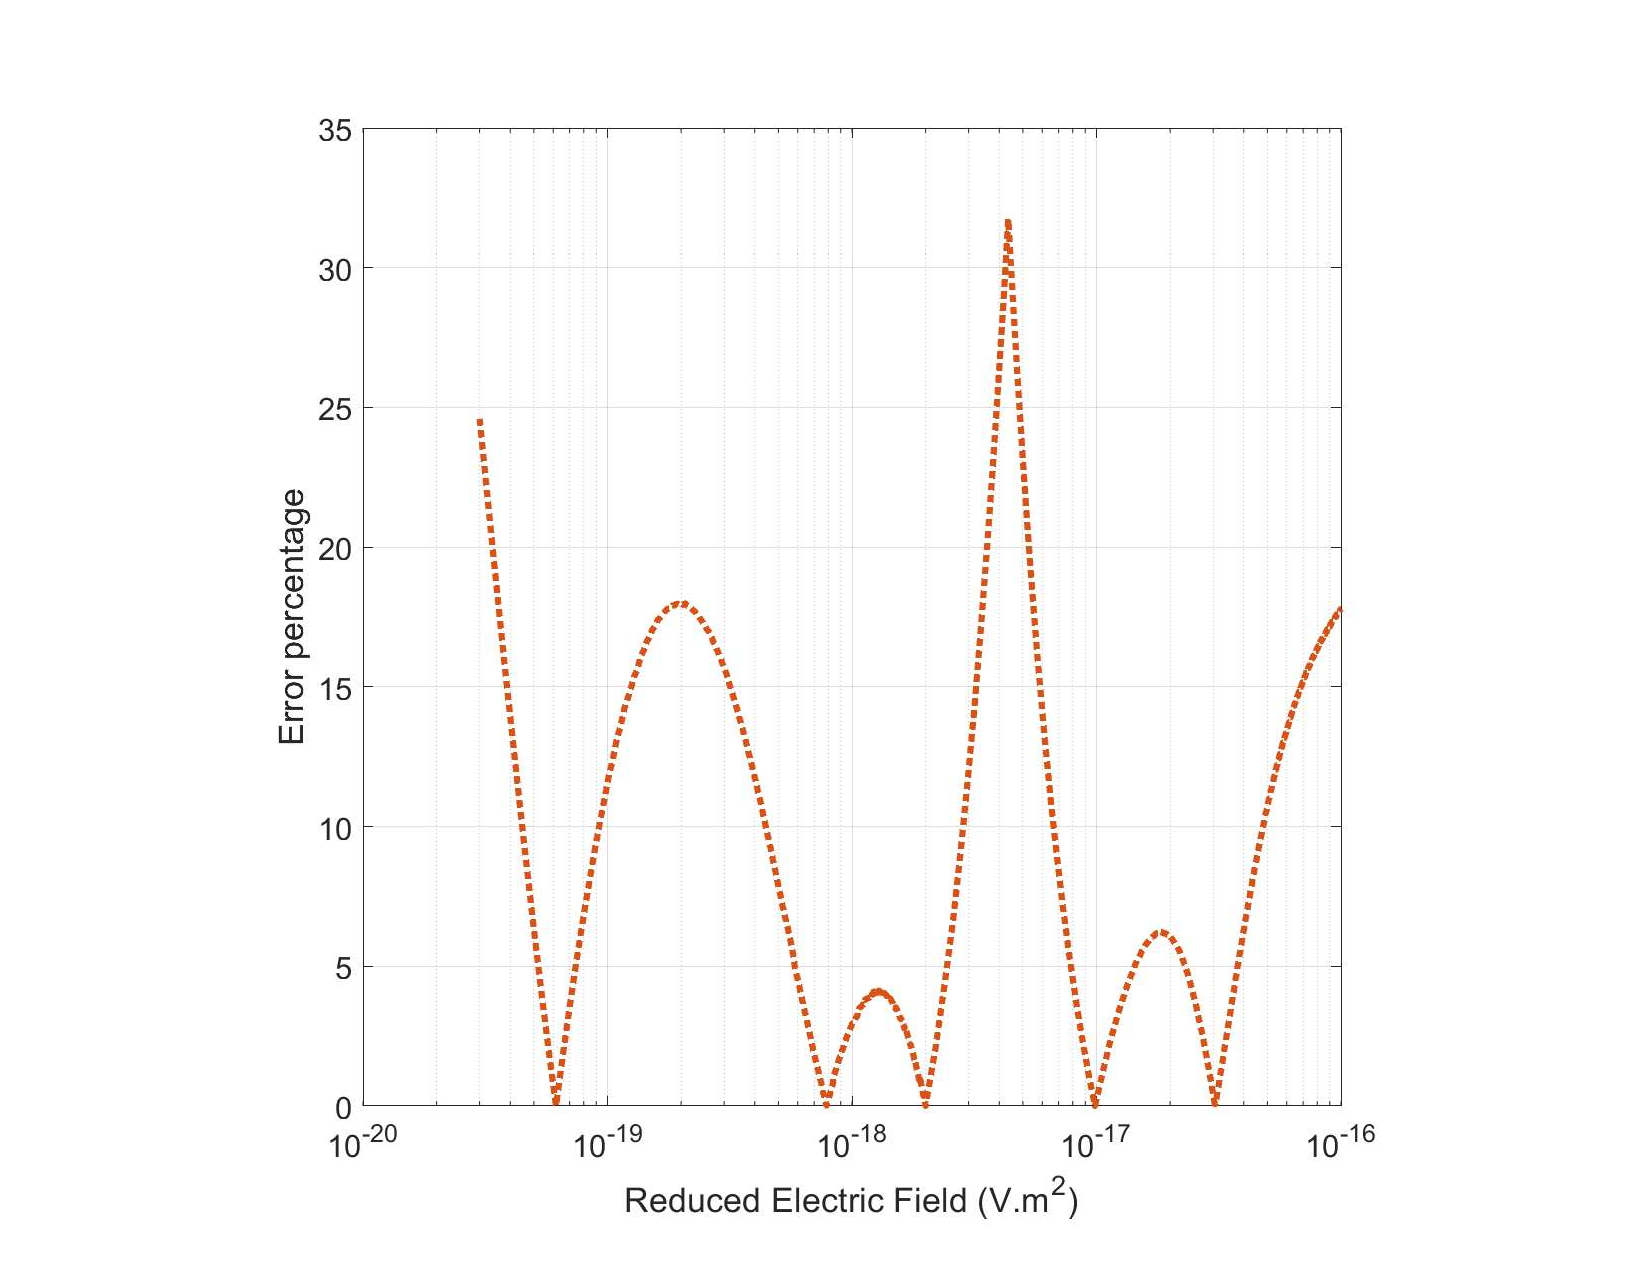
\includegraphics[clip, trim=0.5cm 0.5cm 0.5cm 0.5cm,width=0.95\linewidth]{Reaction_1_2.pdf}}
\caption{Comparison of Reaction 1 rate coefficient (a) Comparison between BOLSIG+ and curve-fit (b) Error percentage of curve-fit when compared with BOLSIG+ data}
\label{fig:Reaction_1_comparison}
\end{figure}
%
%
\begin{figure}[H]
\centering     %%% not \center
\subfigure[]{\label{fig:a}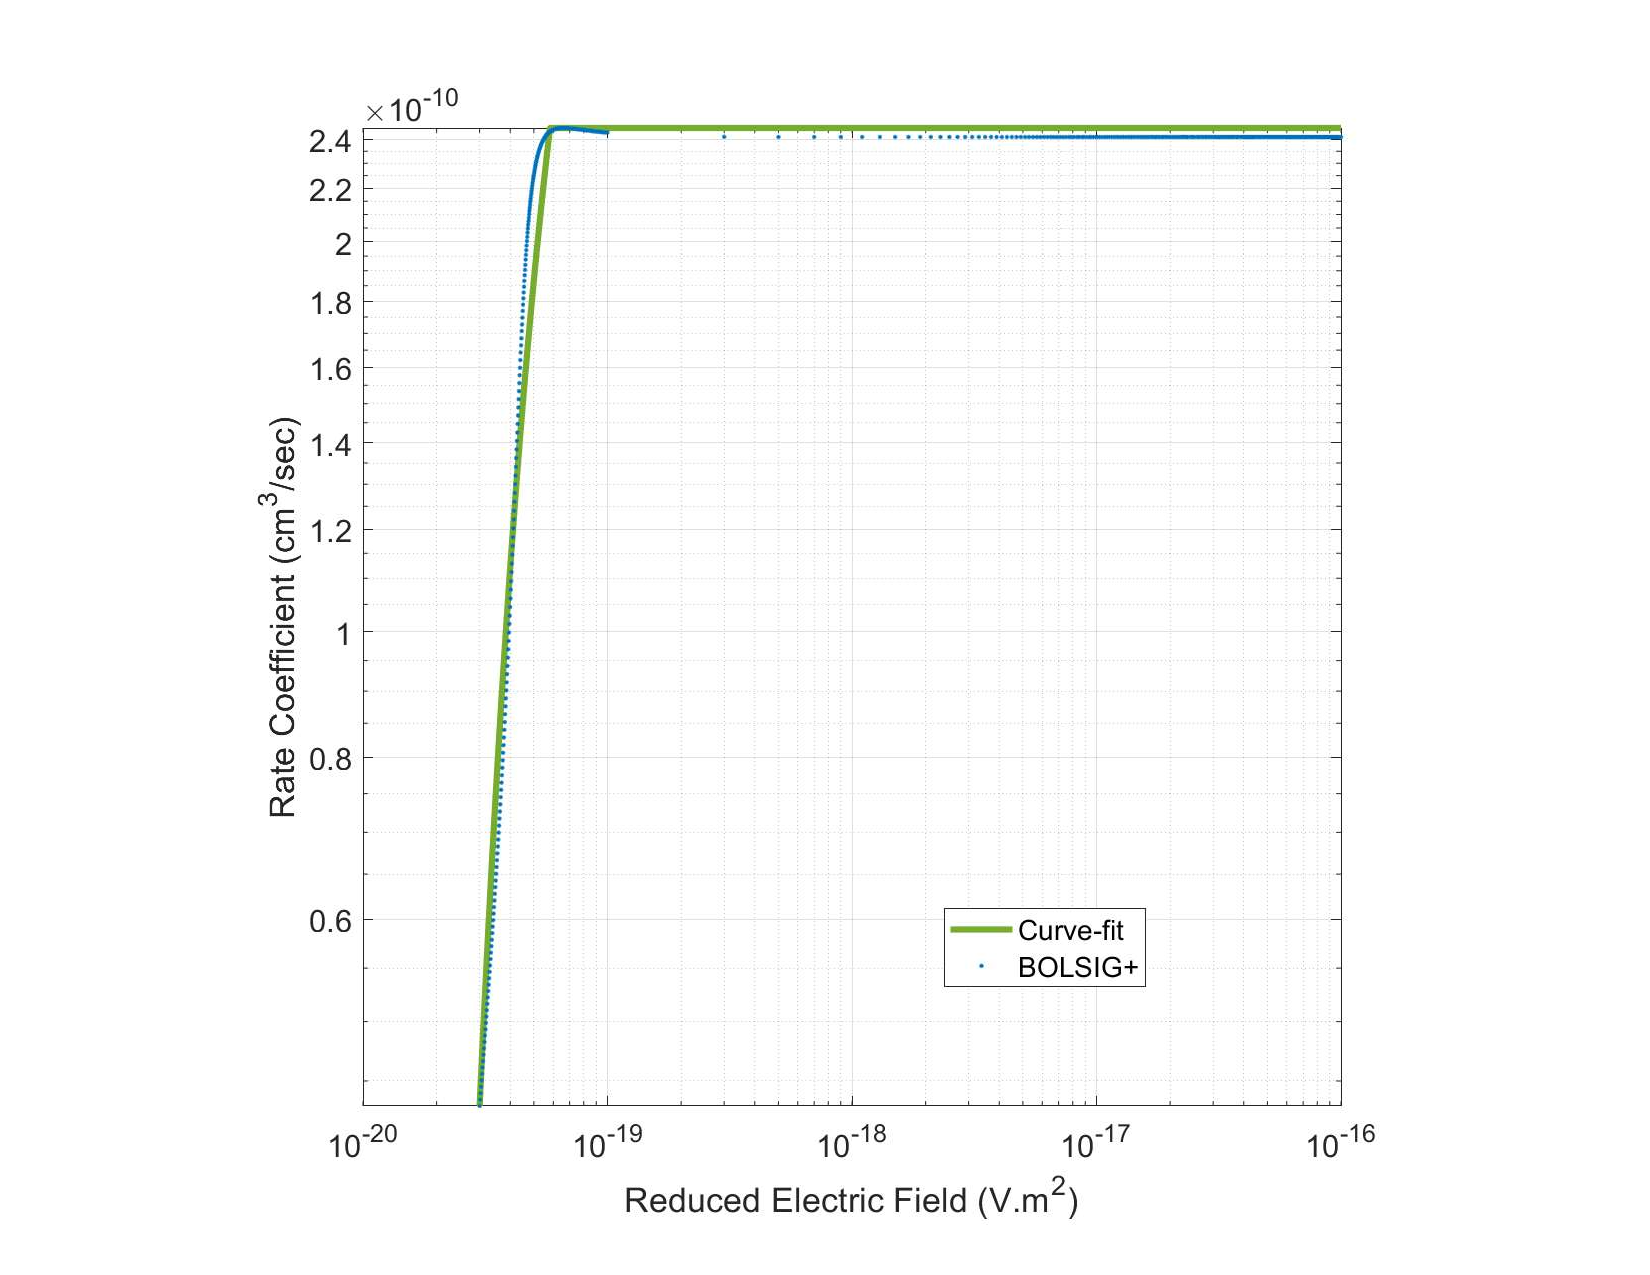
\includegraphics[clip, trim=0.5cm 0.5cm 0.5cm 0.5cm,width=0.95\linewidth]{Reaction_2_1.pdf}}
\subfigure[]{\label{fig:b}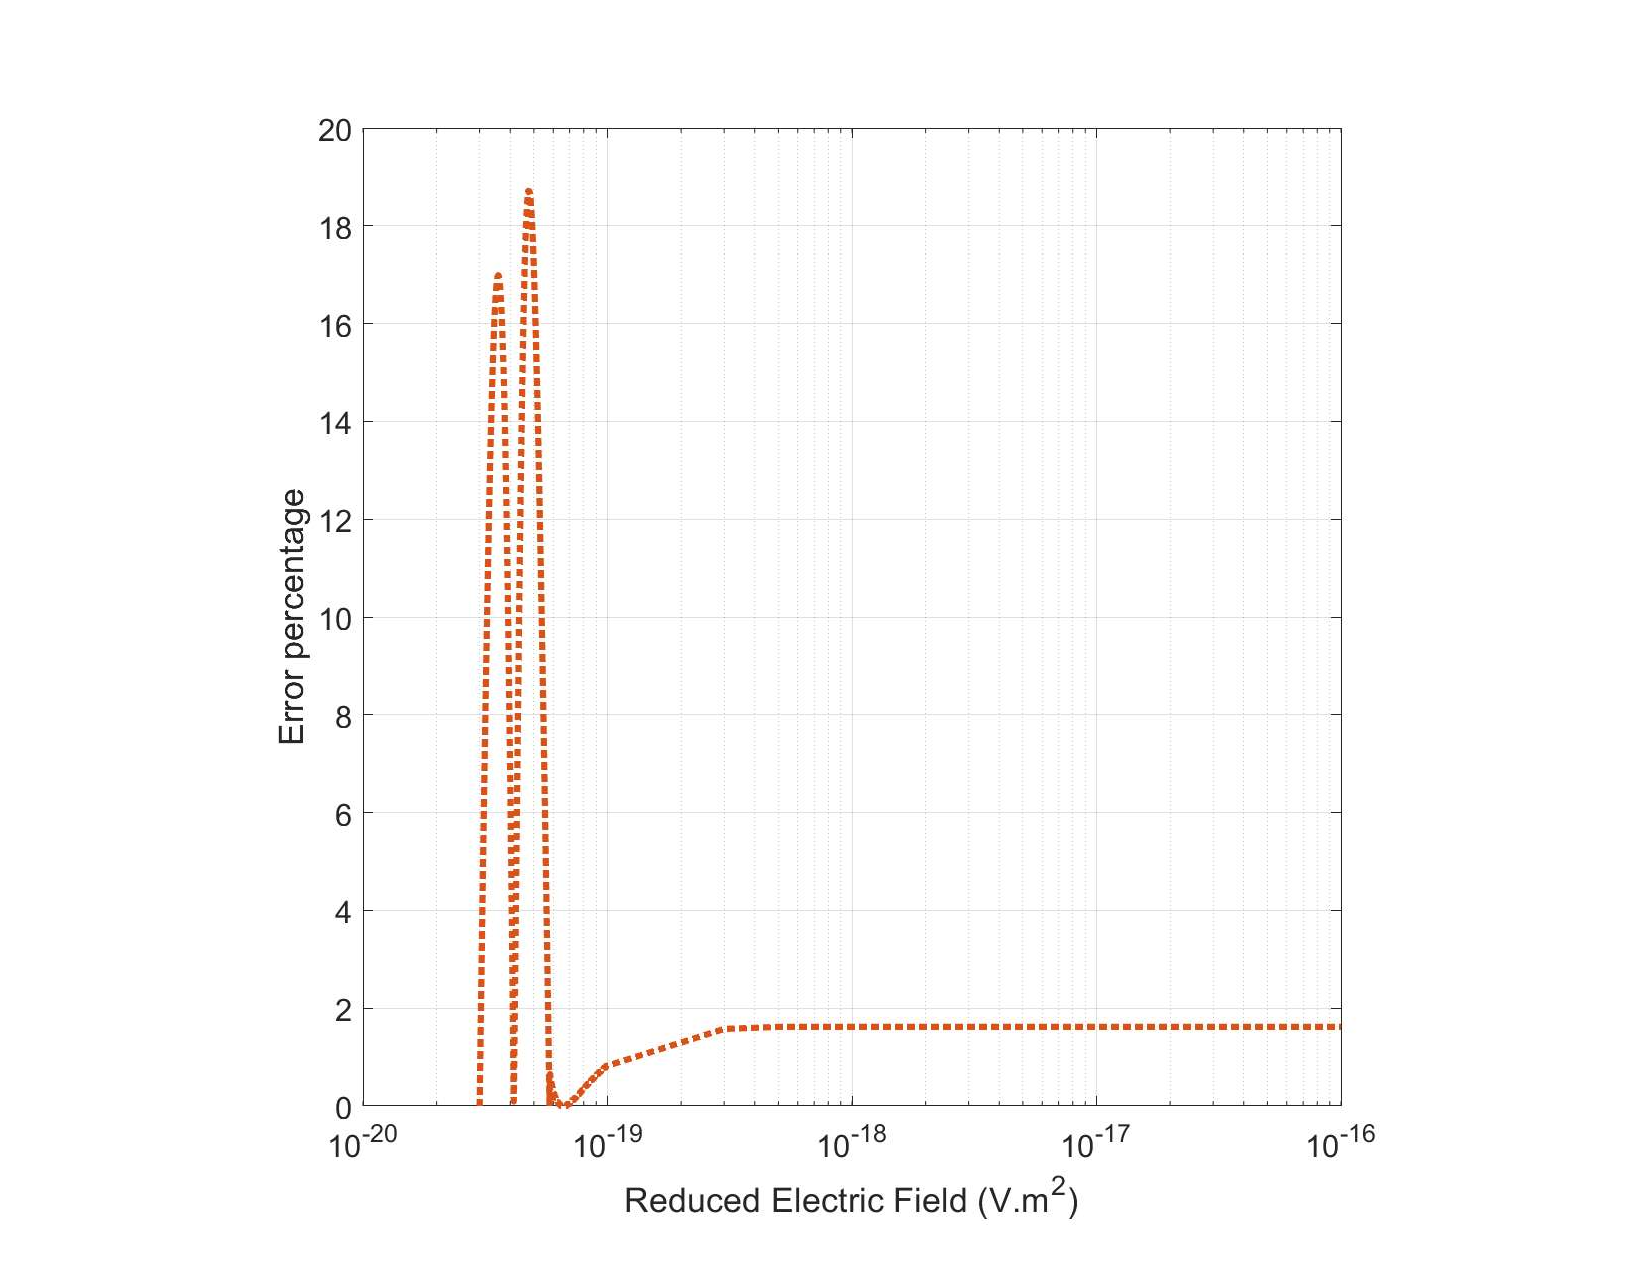
\includegraphics[clip, trim=0.5cm 0.5cm 0.5cm 0.5cm,width=0.95\linewidth]{Reaction_2_2.pdf}}
\caption{Comparison of Reaction 2 rate coefficient (a) Comparison between BOLSIG+ and curve-fit (b) Error percentage of curve-fit when compared with BOLSIG+ data}
\label{fig:Reaction_2_comparison}
\end{figure}
%
%
\begin{figure}[H]
\centering     %%% not \center
\subfigure[]{\label{fig:a}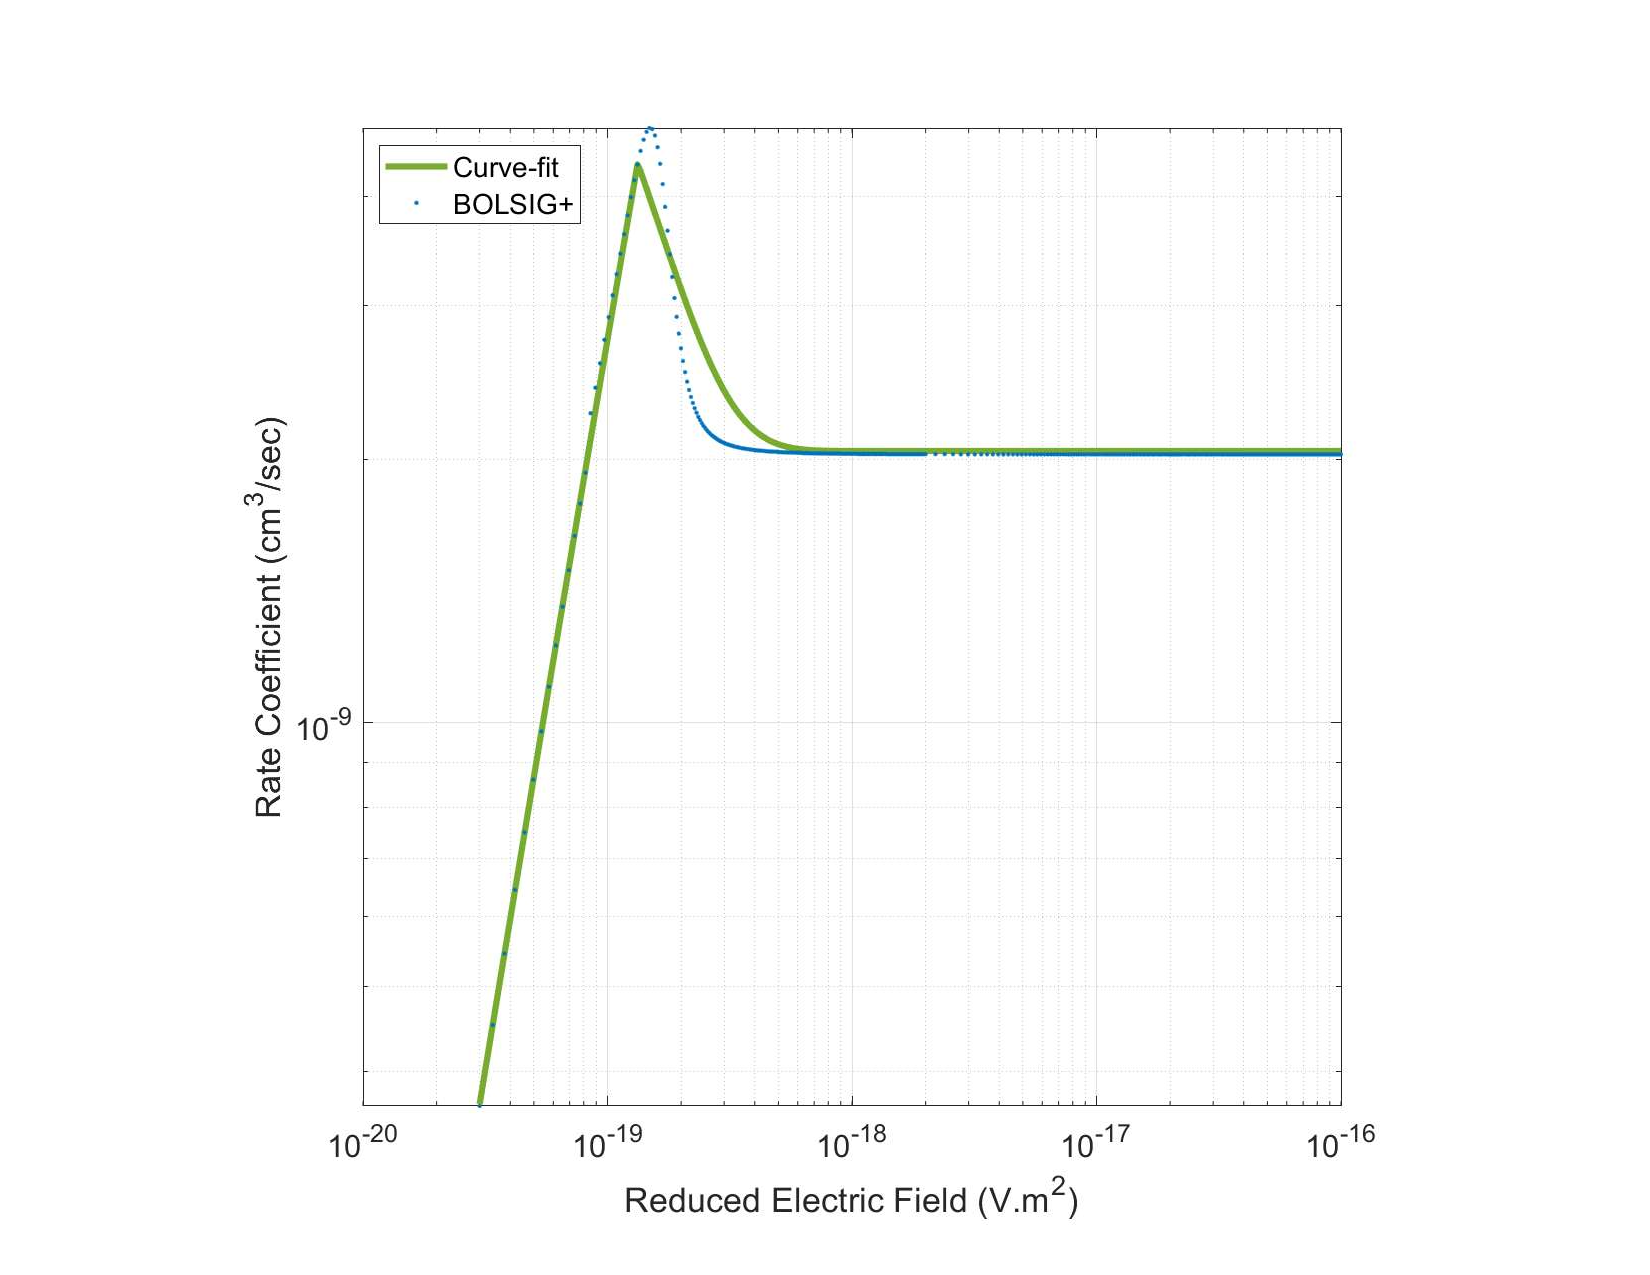
\includegraphics[clip, trim=0.5cm 0.5cm 0.5cm 0.5cm,width=0.95\linewidth]{Reaction_3_1.pdf}}
\subfigure[]{\label{fig:b}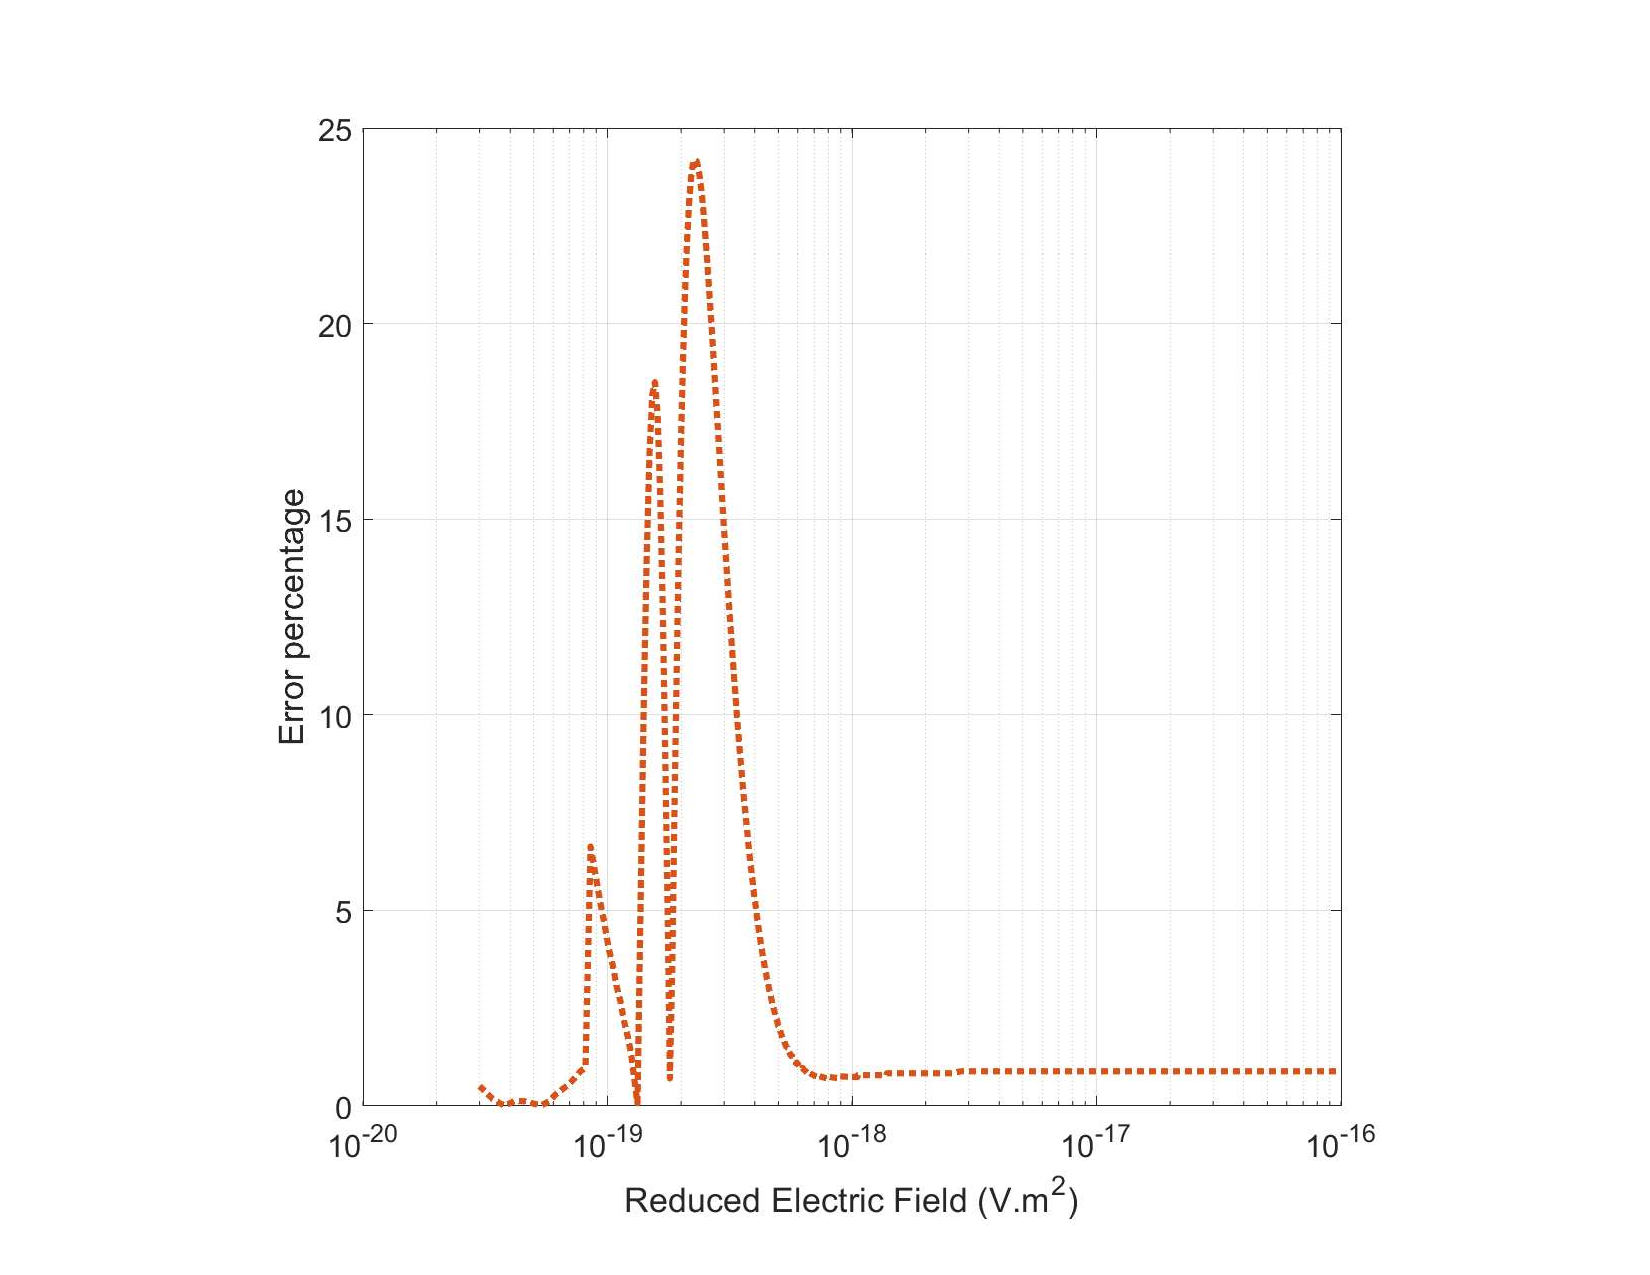
\includegraphics[clip, trim=0.5cm 0.5cm 0.5cm 0.5cm,width=0.95\linewidth]{Reaction_3_2.pdf}}
\caption{Comparison of Reaction 3 rate coefficient (a) Comparison between BOLSIG+ and curve-fit (b) Error percentage of curve-fit when compared with BOLSIG+ data}
\label{fig:Reaction_3_comparison}
\end{figure}
%
%
\begin{figure}[H]
\centering     %%% not \center
\subfigure[]{\label{fig:a}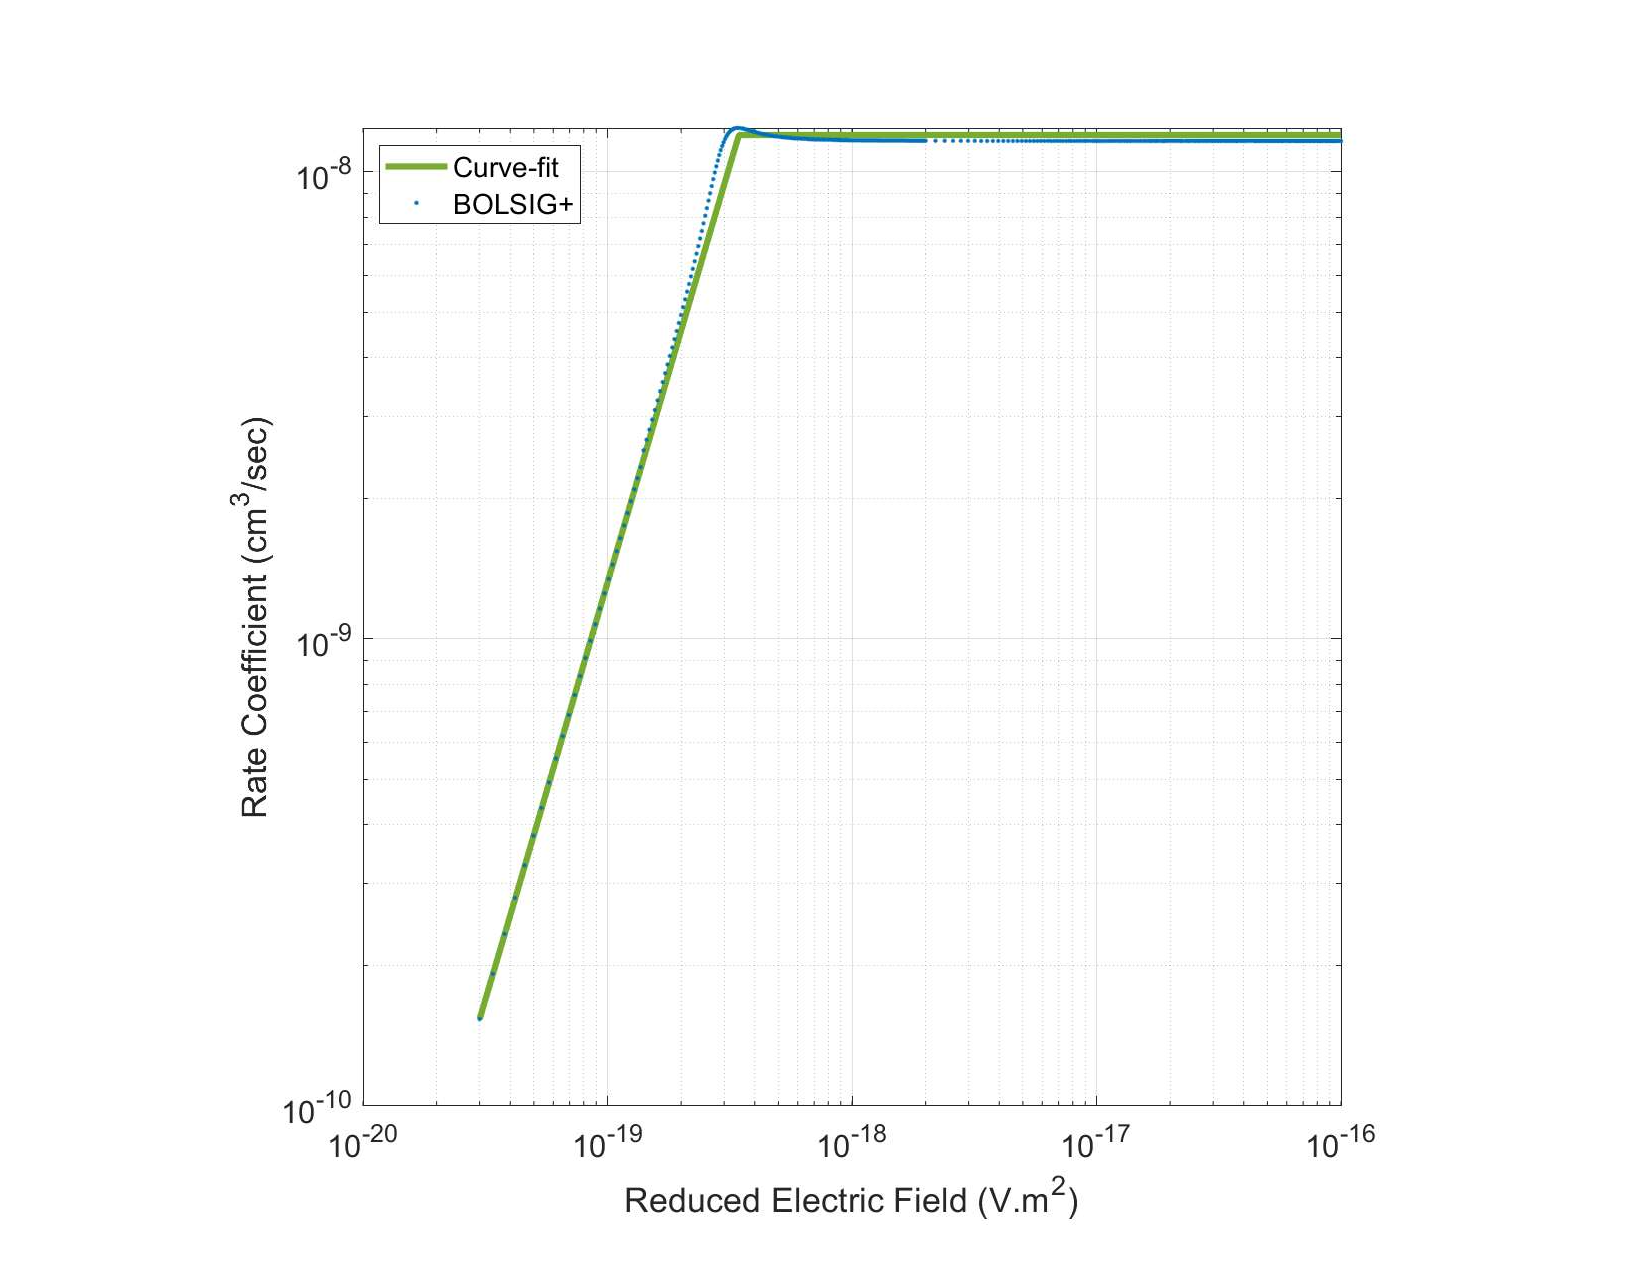
\includegraphics[clip, trim=0.5cm 0.5cm 0.5cm 0.5cm,width=0.95\linewidth]{Reaction_4_1.pdf}}
\subfigure[]{\label{fig:b}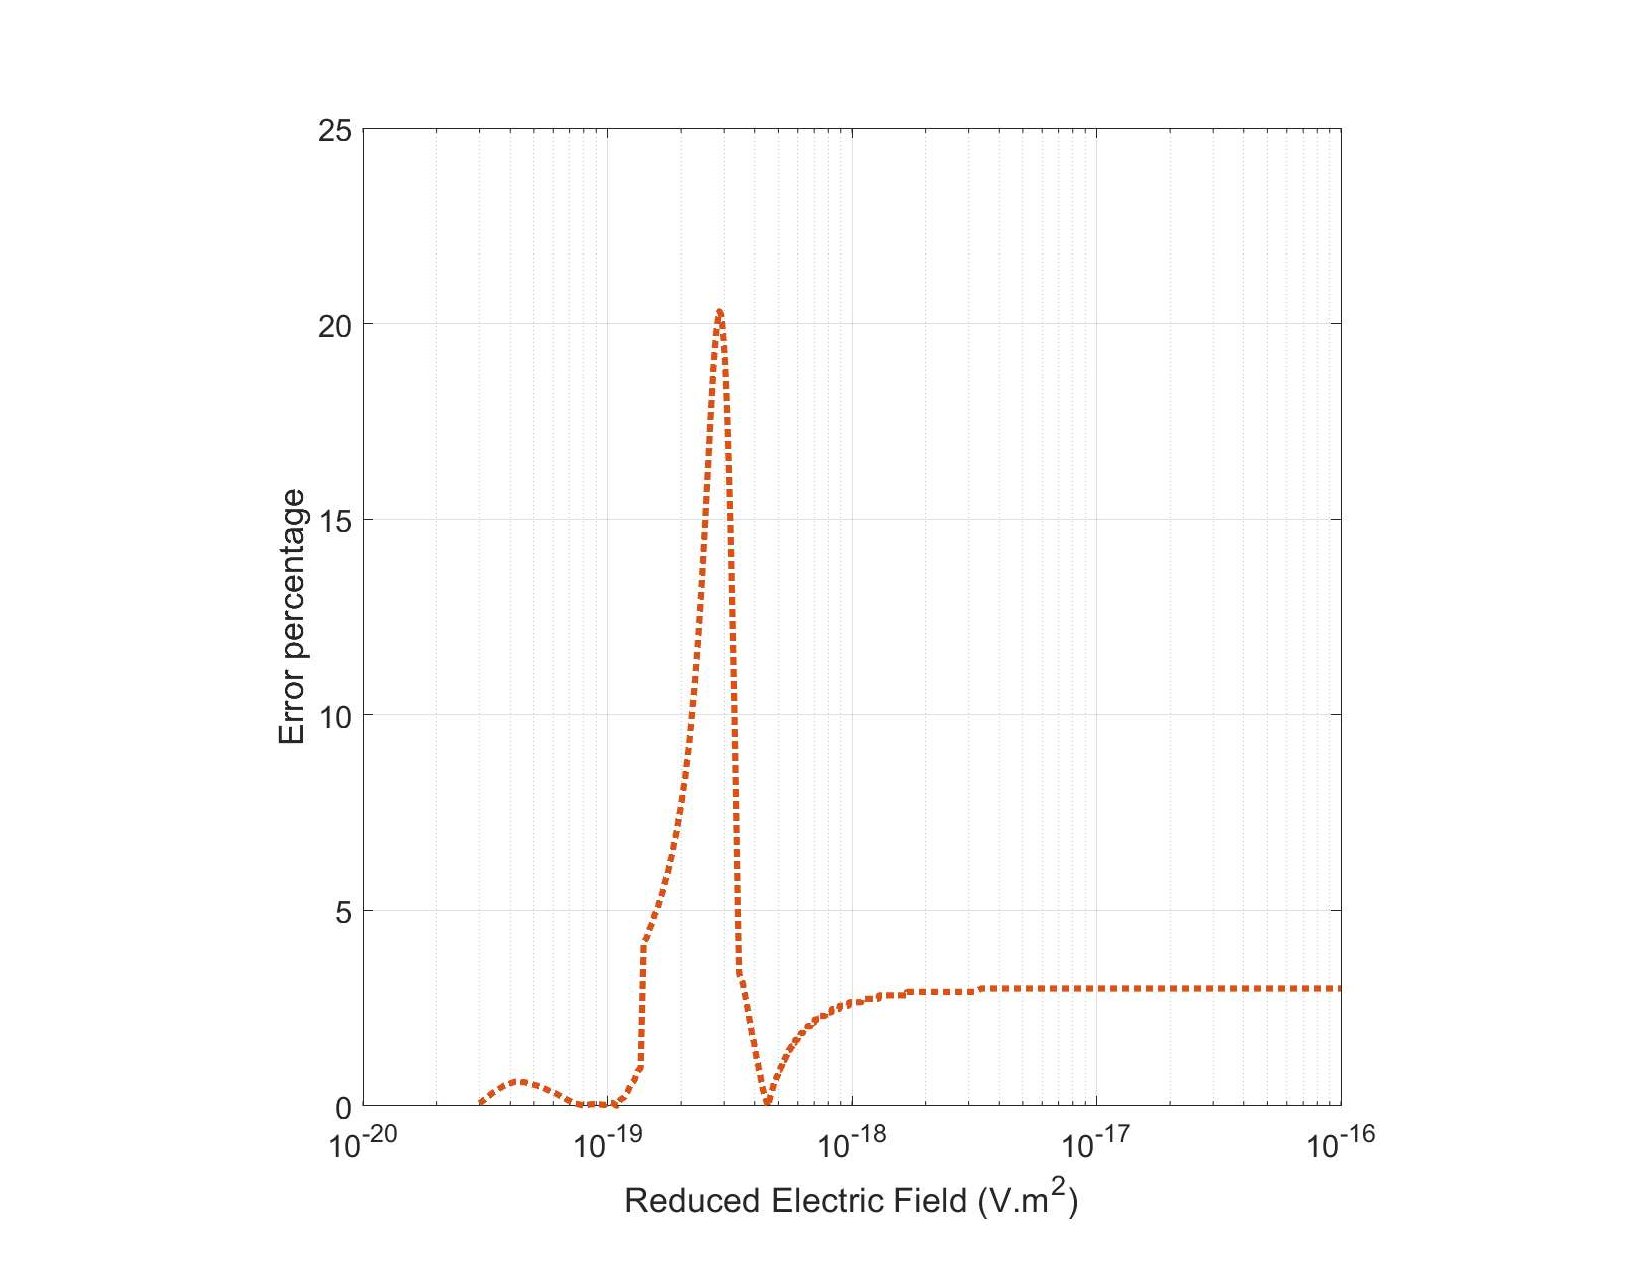
\includegraphics[clip, trim=0.5cm 0.5cm 0.5cm 0.5cm,width=0.95\linewidth]{Reaction_4_2.pdf}}
\caption{Comparison of Reaction 4 rate coefficient (a) Comparison between BOLSIG+ and curve-fit (b) Error percentage of curve-fit when compared with BOLSIG+ data}
\label{fig:Reaction_4_comparison}
\end{figure}
%

%insert a few newpages here to make sure the refs section follows the tables
~
\newpage



\bibliographystyle{warpdoc}
\bibliography{all}


\end{document}



